\chapter{Methodology}
\label{chap:methodology}

This chapter describes how the models are designed, trained and evaluated.

\section{Overall Workflow}

The project has three streams of work (Figure~\ref{fig:workflow}). The first builds review-level models with TensorFlow/Keras. The second, added after the instructor's feedback that the models were not deep enough, introduces LLM-assisted labels, keyword lists and DistilBERT for sentiment and aspect analysis. The third builds the game recommendation on Data Stream v2.

\begin{figure}[!htbp]
    \centering
    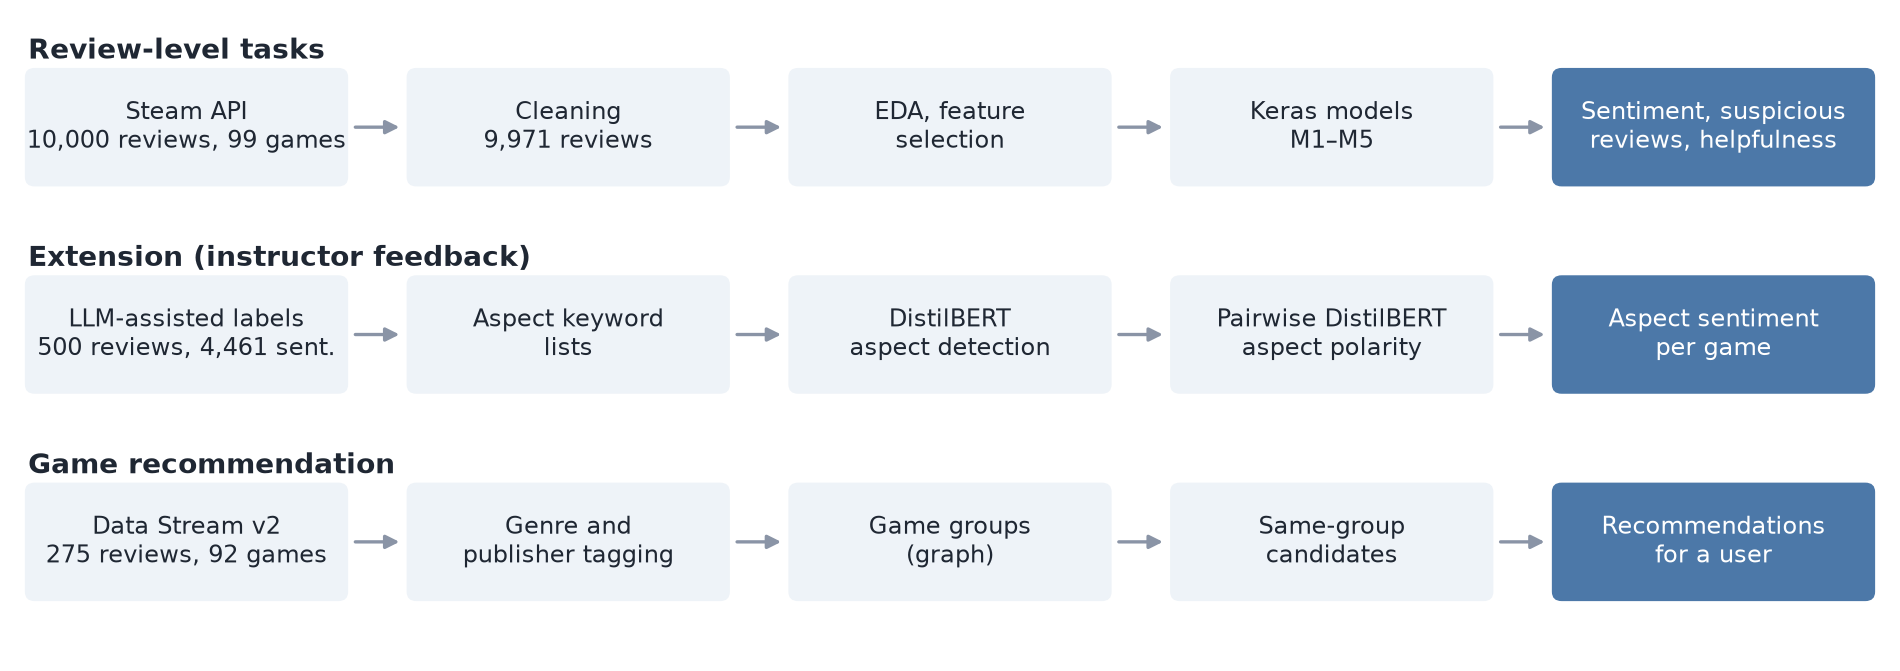
\includegraphics[width=\textwidth]{fig01_workflow.png}
    \caption{Overall workflow of the project.}
    \label{fig:workflow}
\end{figure}

In every experiment, hyperparameters, epochs and thresholds are chosen on the validation (dev) set and the test set is used only for reporting.

\section{Review-Level Models with TensorFlow/Keras}

\subsection{Baselines}

Three logistic regression (LR) baselines show how much information each input carries: \textbf{meta features only} (the ten features of Section~\ref{sec:eda}); \textbf{TF-IDF + LR} with word 1--2-grams (up to 50,000 features) and character 3--5-grams (up to 80,000 features); and \textbf{TF-IDF + meta + LR}. The regularisation strength $C$ is chosen from $\{0.25, \ldots, 8\}$ by validation ROC-AUC.

\subsection{Keras Architectures}

All Keras models share the two-branch structure of Figure~\ref{fig:kerasarch}, built with the functional API. In the \textbf{text branch}, a \texttt{TextVectorization} layer inside the model turns the raw string into token indices (256 tokens cover about 96\% of reviews in full) or into a TF-IDF vector. The \textbf{meta branch} normalises the ten meta features. The branches are concatenated and followed by a dense layer, dropout and a sigmoid output. Because vectorisation is part of the model, a saved \texttt{.keras} file accepts raw text.

\begin{figure}[!htbp]
\centering
\begin{tikzpicture}[
    node distance=0.35cm and 0.6cm,
    box/.style={rectangle, rounded corners=2pt, draw=black!60, fill=blue!8, minimum width=3.2cm, minimum height=0.65cm, align=center, font=\footnotesize},
    var/.style={box, fill=orange!15},
    io/.style={box, fill=gray!12, font=\footnotesize\bfseries},
    arr/.style={-{Stealth[length=2mm]}, thick, black!70}]
\node[io] (txt) {Review text (string)};
\node[box, below=of txt] (vec) {TextVectorization};
\node[var, below=of vec] (enc) {Text encoder M1--M4};
\node[io, right=0.7cm of txt] (meta) {10 meta features};
\node[box, below=of meta] (norm) {Normalization};
\node[box, below=of norm] (md) {Dense(16, ReLU)};
\node[box, below=0.8cm of $(enc)!0.5!(md)$] (cat) {Concatenate};
\node[box, below=of cat] (d32) {Dense(32) + Dropout(0.4)};
\node[io, below=of d32] (out) {Dense(1, sigmoid)};
\draw[arr] (txt) -- (vec); \draw[arr] (vec) -- (enc);
\draw[arr] (meta) -- (norm); \draw[arr] (norm) -- (md);
\draw[arr] (enc) |- (cat); \draw[arr] (md) |- (cat);
\draw[arr] (cat) -- (d32); \draw[arr] (d32) -- (out);
\node[font=\scriptsize, right=0.35cm of md, draw=black!30, rounded corners=2pt, inner sep=3pt, anchor=west] {%
\renewcommand{\arraystretch}{1.1}%
\begin{tabular}{@{}l@{\ }l@{}}
\textbf{M1:} & Embedding(64) $\rightarrow$ GlobalAvgPool \\
\textbf{M2:} & Embedding(64) $\rightarrow$ BiLSTM(64) \\
\textbf{M3:} & Embedding(64) $\rightarrow$ Conv1D(128, 5) $\rightarrow$ MaxPool \\
\textbf{M4:} & TF-IDF (30k) $\rightarrow$ Dropout(0.5) $\rightarrow$ Dense(32) \\
\textbf{M5:} & mean of the M2 and M4 outputs
\end{tabular}};
\end{tikzpicture}
\caption{Two-branch architecture shared by the Keras models.}
\label{fig:kerasarch}
\end{figure}

The models differ only in the text encoder (legend of Figure~\ref{fig:kerasarch}), following the text-classification labs of the course. M1 ignores word order, M2 captures order and negation, and M3 detects local phrases. M4 was added because M1--M3 did not beat the TF-IDF baseline: it brings n-gram TF-IDF features into a Keras network. M5 averages M2 and M4, which read the text differently (prediction correlation 0.85). Each model is trained separately for scenarios A and B.

\subsection{Suspicious Review Detection}

There are no labels for spam, trolling or sarcasm, so suspicious reviews are found from the disagreement between content and verdict, plus the quality rules (Algorithm~\ref{alg:suspicious}). M4 is trained in 5-fold cross-validation so that every review is scored by a model that has not seen it. The output is a ranked list of candidates for human review, not an automatic spam filter.

\begin{algorithm}[!htbp]
\caption{Suspicious review detection}
\label{alg:suspicious}
\begin{algorithmic}[1]
\For{each of 5 stratified folds $k$}
    \State Train M4 on the other folds; predict $p_i = P(\text{positive} \mid \text{text}_i)$ for reviews in fold $k$
\EndFor
\For{each review $i$ with Steam label $y_i$}
    \State $\text{mismatch}_i \gets (y_i = 0 \land p_i \geq 0.9) \lor (y_i = 1 \land p_i \leq 0.1)$
    \State $\text{suspicion}_i \gets |y_i - p_i|$ \Comment{0 = consistent, 1 = opposite}
    \State $\text{suspicious}_i \gets \text{mismatch}_i \lor \text{any quality flag}_i$
\EndFor
\State \textbf{return} suspicious reviews ranked by suspicion score
\end{algorithmic}
\end{algorithm}

The thresholds 0.9 and 0.1 keep only confident disagreements; reviews with $p$ close to 0.5 are reported separately as ``uncertain''.

\subsection{Helpfulness Prediction}

The target is whether a review had at least one helpful vote at crawl time (32.5\% of reviews), an observed label rather than a validated forecast of future votes; a binary target is used because 67.5\% of reviews have no vote. Older reviews have had more time to collect votes, so the log review age in days is added as a control variable. Inputs are the text, the meta features, review age and the sentiment label. Four models are compared: LR on age only, LR on meta features and age, TF-IDF + meta + age with LR, and Keras M4 on the same inputs with class weights for the minority class.

\section{Transformer Models}

\subsection{DistilBERT for Review Sentiment}

The pre-trained \texttt{distilbert-base-uncased} \cite{Sanh2019} is fine-tuned through Keras 3 and KerasHub. Inputs are limited to 128 tokens; for longer reviews the first and last parts are kept \cite{SunFinetune2019}, since reviewers often state their conclusion at the end. Token vectors are averaged (padding masked), followed by dropout 0.2 and a sigmoid output. The model uses the same splits as the Keras models, in both scenarios, with three seeds.

\subsection{Aspect Detection}

Aspect detection has eight sigmoid outputs, one per aspect, each with its own threshold chosen on dev. Five methods are compared: \textbf{keywords} (hand-written regular expressions per aspect, e.g. \texttt{crash|lag|fps} for performance), \textbf{TF-IDF + LR} (one balanced logistic regression per aspect), \textbf{DistilBERT} fine-tuned with eight outputs, the \textbf{union} of keywords and DistilBERT, and \textbf{keywords-in-input}. In the last method, the aspects found by the keywords are written before the sentence, \texttt{[CLS] graphics price [SEP] sentence [SEP]}, and DistilBERT decides whether to trust these hints, combining the precision of keywords with the transformer's ability to recognise paraphrases.
To measure the effect of labelled data, keywords-in-input is trained on 1,265, 1,995, 2,725 and 2,913 sentences, and plain DistilBERT on the smallest and largest sizes.

\subsection{Pairwise Aspect Polarity}

For each (sentence, aspect) pair the model receives \texttt{[CLS] aspect [SEP] sentence [SEP]}, with the aspect as one word (``graphics'', ``performance'', \ldots), and predicts whether that aspect is praised or criticised \cite{SunABSA2019}. A sentence with two aspects thus gets two independent predictions. Only pairs whose gold polarity is positive or negative are used, so this is a binary task. The encoder is initialised from a DistilBERT sentiment model fine-tuned on Steam labels, so it starts with knowledge of game-review sentiment. To target the hardest case, one training variant adds 188 sentences with a contrastive connective (``but'', ``however'') and at least two aspects. The baselines give every aspect of a sentence the sentence's polarity, predicted by M4 or by sentence-level DistilBERT.

\subsection{End-to-End Aspect Pipeline}

A review is split into sentences at sentence-ending punctuation and line breaks (keeping sentences of at least three words); each sentence goes through aspect detection, every detected aspect is scored by the pairwise model, and the pairs are aggregated per game (Figure~\ref{fig:absapipe}).

\begin{figure}[!htbp]
\centering
\begin{tikzpicture}[
    node distance=0.3cm,
    box/.style={rectangle, rounded corners=2pt, draw=black!60, fill=blue!8, minimum height=1.1cm, text width=1.9cm, align=center, font=\footnotesize},
    hl/.style={box, fill=orange!15, text width=2.5cm},
    arr/.style={-{Stealth[length=2mm]}, thick, black!70}]
\node[box] (r) {Review text};
\node[box, right=of r] (s) {Split into sentences};
\node[hl, right=of s] (d) {Aspect detection\\(keyword hints)};
\node[hl, right=of d] (p) {Pairwise polarity per aspect};
\node[box, right=of p] (g) {Aggregate per game};
\draw[arr] (r) -- (s); \draw[arr] (s) -- (d); \draw[arr] (d) -- (p); \draw[arr] (p) -- (g);
\end{tikzpicture}
\caption{End-to-end aspect-based sentiment pipeline.}
\label{fig:absapipe}
\end{figure}

\section{Game Recommendation}

Every user in Data Stream v2 wrote one review, so collaborative filtering, which needs users who rated several games, is not possible. A content-based method is used instead: games are compared by their attributes. Games, genres and publishers with at least two games form a graph in which each game is linked to its genre and publisher. For a user who liked game $g$, every other game $h$ is scored as
\begin{equation}
    \text{score}(h) = 2 \cdot \mathbf{1}[\text{genre}(h) = \text{genre}(g)] + \mathbf{1}[\text{publisher}(h) = \text{publisher}(g)],
\end{equation}
with ties broken by the overall positive rating of $h$. Genre has the larger weight because players usually look for the same type of game. If the user disliked $g$, highly rated games from other genres are suggested.

\section{Hyperparameters and Implementation}

Table~\ref{tab:hparams} lists the training settings. Transformers are scored on dev after each epoch and the best epoch is kept.

\begin{table}[!htbp]
\centering
\caption{Training configuration}
\label{tab:hparams}
\small
\begin{tabularx}{\textwidth}{lYY}
\toprule
\textbf{Setting} & \textbf{Keras models (M1--M4)} & \textbf{DistilBERT models} \\
\midrule
Optimizer & Adam & AdamW, weight decay 0.01, gradient clipping 1.0 \\
Learning rate & $10^{-3}$ ($3 \times 10^{-4}$ for M4) & $2 \times 10^{-5}$ ($3 \times 10^{-5}$ for aspect detection), 10\% warm-up, cosine decay \\
Batch size & 64 & 16 \\
Epochs & up to 15 (30 for M1), early stopping (patience 2) & 3 (sentiment), 6 (aspect detection), 5 (polarity) \\
Input length & 256 tokens, vocabulary 20,000 & 128 tokens, head + tail truncation \\
Regularisation & Dropout 0.4 (0.5 in M4), L2 $10^{-4}$ in M4 & Dropout 0.2 \\
Seeds & 1 & 3 (2 for some aspect variants) \\
\bottomrule
\end{tabularx}
\end{table}

The implementation uses Python 3.12 with pandas, NumPy, Matplotlib and \textbf{scikit-learn} (TF-IDF, LR baselines, splits, metrics). Keras models M1--M5 and the helpfulness model use \textbf{TensorFlow/Keras 2.20} on CPU (20--75 seconds per model). DistilBERT is fine-tuned with \textbf{Keras 3 and KerasHub on the PyTorch backend} on an NVIDIA GTX 1650 (4~GB), because recent TensorFlow versions do not support GPUs on native Windows (about 10 minutes per sentiment run, 2.5 hours for the final aspect experiment). A local \textbf{web application} (FastAPI and HTML/JavaScript) serves the Keras models of Tasks 1--3 and the recommendation (single-review analysis, batch moderation, data overview); the transformer checkpoints are not yet integrated into it.
